\documentclass[a4paper]{article}
\author{Kim Rune Solstad}
\title{Assignment 5}
\usepackage{enumerate}
\usepackage{listings}
\usepackage{graphicx}
\begin{document}
\maketitle
\section{Introduction}
For this assignment, I modified the program delivered for assignment 4.
A solution where there could be more than one queen per line where attempted, but not sucsessfully created. However the program is able to solve 30 - queens problem in a couple of secounds. 

\section{The algorithm}
The algorithm implemented in the new solution is a local-search with constraint reasoning. First, a state is generated with partially randomized queens. Each row gets K-queens. Each domain in one column is then given a value that represents the numer of conflicts a potential queen would face if placed there. The queens in the selected column is then placed in the domains with the lowest amount of potential conflicts. This process is repeated until all columns are visited. The state is then evaluated. If none conflicts are found, a winner-state is returned. If conficts are found, the process repeat starting with the first column.
\\
The algorithm stagnates when conflicts are found, but better domains for the queens are not. To detect stagnation, a counter is increased for each state generated, (that is not randomized), without decreasing the amount of conflicts. When this counter reach the max-value, 6 in this case, the state gets randomized.

\section{Instructions} 
Compile all files in src with javac. 
\\' javac *.java ' \\
Run Test.class with java. Use option 'a' for algorithm. Use option 'n' to decide amount of queens. Use 'v' to display extra info.
\\ ' java Test \{[option]\}' \\
To run with 16 queens:
\\ ' java Test a n16 ' \\

\section{Output}
\subsection{8-queen}
Example output from 8-queen puzzle:
\lstinputlisting{output_8-queen.txt}
Average time to complete 8-queen puzzle is 0.278 sek. 
\subsection{16-queen}
Example output from 16-queen puzzle:
\lstinputlisting{output_16-queen.txt}
Average time to complete 16-queen puzzle is 0.416 sek.

\section{Plot}
The graph shows average time spent on solving puzzles with different number of queens. 32 queens took an average of 6 secounds.
\\
\centerline{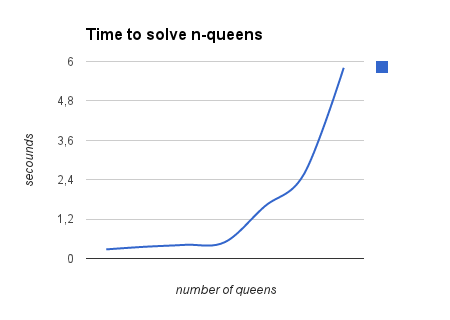
\includegraphics{diagram1.png}}

\section{Changelog}
\begin{enumerate}
	\item Egg randomizing code moved from State.java to separate class called EggCartonEggRandomizer.java.
	\item New eggrandomizing class created. This one places k eggs in each row of carton. This code is to be found in EggCartonRandomizer\_v2.java
	\item EggCartonObjectiveFunction.java has been supplemented with a method that counts obstacles in a single domain
	\item MinConflictLocalSearchPuzzleSolver.java added. Constraint satisfying algorithm to solve n-queens puzzle. 

\end{enumerate}
\end{document}

